%%%%%%%%%%%%%%%%%%%%%%%%%%%%%%%%%%%%%%%%%
% CN2 Labreport template
%
% License:
% CC BY-NC-SA 3.0 (http://creativecommons.org/licenses/by-nc-sa/3.0/)
%
%%%%%%%%%%%%%%%%%%%%%%%%%%%%%%%%%%%%%%%%%

\documentclass[parskip=full]{scrartcl}

\usepackage{siunitx}  % Provides the \SI{}{} command for typesetting SI units
\usepackage{graphicx} % Required for the inclusion of images
\usepackage{booktabs} % nicer tables
\usepackage[noabbrev]{cleveref} % automatic references
\usepackage{listings} % typeset code

\crefname{lstlisting}{listing}{listings} % for referencing code
\Crefname{lstlisting}{Listing}{Listings} % for referencing code

\usepackage[headsepline]{scrlayer-scrpage} % header
\ohead{Group 08} % right part of header
\ihead{Assignment 3} % left part of header

\lstset{basicstyle=\ttfamily} % monospaced font in listing

\usepackage{lstautogobble}  % Fix relative indenting
\usepackage{color}          % Code coloring
\usepackage{zi4}            % Nice font

\definecolor{bluekeywords}{rgb}{0.13, 0.13, 1}
\definecolor{greencomments}{rgb}{0, 0.5, 0}
\definecolor{redstrings}{rgb}{0.9, 0, 0}
\definecolor{graynumbers}{rgb}{0.5, 0.5, 0.5}

\usepackage{listings}
\lstset{
    autogobble,
    columns=fullflexible,
    showspaces=false,
    showtabs=false,
    breaklines=true,
    showstringspaces=false,
    breakatwhitespace=true,
    escapeinside={(*@}{@*)},
    commentstyle=\color{greencomments},
    keywordstyle=\color{bluekeywords},
    stringstyle=\color{redstrings},
    numberstyle=\color{graynumbers},
    basicstyle=\ttfamily\footnotesize,
    frame=l,
    framesep=12pt,
    xleftmargin=12pt,
    tabsize=4,
    captionpos=b
}



%----------------------------------------------------------------------------------------
%	DOCUMENT INFORMATION
%----------------------------------------------------------------------------------------

\begin{document}
\begin{titlepage}
    \centering
    \vspace*{2cm}
    {\Huge \textbf{Communication Networks 2}}\\
    SS 2017\\
    \vspace*{1cm}
    {\Large Assignment 3}
    \\\vspace*{3cm}
    {\Large \textbf{Group 08}}\\
    \vspace*{1cm}
    {\large 
        \begin{tabular}{l c c}
            Name & Mat.Nummer \\ \hline
            Constantin SCHIEBER & 01228774 \\
            Andreas HIRTENLEHNER & 01327273
        \end{tabular}
    }
    \\\vspace*{7cm}
    \today
\end{titlepage}

%----------------------------------------------------------------------------------------
%	SECTION 1
%----------------------------------------------------------------------------------------
\section{Network Hierarchy Recovery}

\begin{verbatim}
traceroute to landline.cn2lab.cn.tuwien.ac.at (10.1.6.110), 30 hops max, 60 byte packets
 1  border.cn2lab.cn.tuwien.ac.at (192.168.88.2)  6.382 ms  6.279 ms  6.259 ms
 2  10.0.20.1 (10.0.20.1)  322.040 ms  326.126 ms  326.109 ms
 3  landline.cn2lab.cn.tuwien.ac.at (10.1.6.110)  326.091 ms  326.073 ms  326.055 ms
\end{verbatim}

\begin{verbatim}
traceroute to satellite.cn2lab.cn.tuwien.ac.at (10.1.7.123), 30 hops max, 60 byte packets
 1  border.cn2lab.cn.tuwien.ac.at (192.168.88.2)  3.160 ms  3.286 ms  3.250 ms
 2  10.0.20.1 (10.0.20.1)  155.870 ms  160.159 ms  161.802 ms
 3  10.0.84.2 (10.0.84.2)  2685.357 ms  2692.193 ms  2692.169 ms
 4  satellite.cn2lab.cn.tuwien.ac.at (10.1.7.123)  2692.266 ms  2692.375 ms  2692.533 ms
\end{verbatim}

\begin{verbatim}
CN_08@pc05:~$ ip -6 neigh
fe80::1ec1:deff:fe80:3261 dev eno1 lladdr 1c:c1:de:80:32:61 router REACHABLE
2001:629:2600:a018::2 dev eno1 lladdr 72:8f:5d:f9:92:6f router STALE
fe80::708f:5dff:fef9:926f dev eno1 lladdr 72:8f:5d:f9:92:6f router STALE
2001:629:2600:a018::1 dev eno1 lladdr 1c:c1:de:80:32:61 router STALE
CN_08@pc05:~$ ip -4 neigh
192.168.88.2 dev eno1 lladdr 72:8f:5d:f9:92:6f REACHABLE
192.168.88.1 dev eno1 lladdr 1c:c1:de:80:32:61 REACHABLE
\end{verbatim}

\begin{verbatim}
traceroute to 10.0.84.2 (10.0.84.2), 30 hops max, 60 byte packets
 1  * * *
 2  10.0.20.1 (10.0.20.1)  165.113 ms  165.100 ms  165.091 ms
 3  10.0.84.2 (10.0.84.2)  955.090 ms  955.082 ms  971.120 ms
\end{verbatim}

\begin{verbatim}
Nmap scan report for 10.0.20.2
Nmap scan report for 10.0.84.1
Nmap scan report for 10.0.212.1
Nmap scan report for 10.0.212.52
\end{verbatim}

\begin{verbatim}
CN_08@pc17:~/Downloads/Assignments/3_Assignment$ traceroute 10.0.212.52
traceroute to 10.0.212.52 (10.0.212.52), 30 hops max, 60 byte packets
 1  border.cn2lab.cn.tuwien.ac.at (192.168.88.2)  3.046 ms  3.075 ms  3.323 ms
 2  10.0.212.52 (10.0.212.52)  3.291 ms  3.242 ms  3.207 ms
CN_08@pc17:~/Downloads/Assignments/3_Assignment$ traceroute 10.0.212.1
traceroute to 10.0.212.1 (10.0.212.1), 30 hops max, 60 byte packets
 1  10.0.212.1 (10.0.212.1)  2.846 ms  2.910 ms  3.269 ms
CN_08@pc17:~/Downloads/Assignments/3_Assignment$ traceroute 10.0.84.1
traceroute to 10.0.84.1 (10.0.84.1), 30 hops max, 60 byte packets
 1  10.0.84.1 (10.0.84.1)  3.296 ms  3.208 ms  3.172 ms
CN_08@pc17:~/Downloads/Assignments/3_Assignment$ traceroute 10.0.20.2
traceroute to 10.0.20.2 (10.0.20.2), 30 hops max, 60 byte packets
 1  10.0.20.2 (10.0.20.2)  3.098 ms  3.132 ms  3.117 ms
\end{verbatim}

Own address: 192.168.88.117

\begin{verbatim}
CN_08@pc17:~/Downloads/Assignments/3_Assignment$ ip route get 10.0.212.52
10.0.212.52 via 192.168.88.2 dev eno1 src 192.168.88.117 uid 5007
    cache
CN_08@pc17:~/Downloads/Assignments/3_Assignment$ ip route get 10.0.212.1
10.0.212.1 via 192.168.88.2 dev eno1 src 192.168.88.117 uid 5007
    cache
CN_08@pc17:~/Downloads/Assignments/3_Assignment$ ip route get 10.0.84.1
10.0.84.1 via 192.168.88.2 dev eno1 src 192.168.88.117 uid 5007
    cache
CN_08@pc17:~/Downloads/Assignments/3_Assignment$ ip route get 10.0.20.1
10.0.20.1 via 192.168.88.2 dev eno1 src 192.168.88.117 uid 5007
    cache
\end{verbatim}

\begin{verbatim}
ping -4 landline.cn2lab.cn.tuwien.ac.at
PING landline.cn2lab.cn.tuwien.ac.at (10.1.6.110) 56(84) bytes of data.
64 bytes from landline.cn2lab.cn.tuwien.ac.at (10.1.6.110): icmp_seq=1 ttl=62 time=158 ms
\end{verbatim}

\begin{verbatim}
ping -4 satellite.cn2lab.cn.tuwien.ac.at
PING satellite.cn2lab.cn.tuwien.ac.at (10.1.7.123) 56(84) bytes of data.
64 bytes from satellite.cn2lab.cn.tuwien.ac.at (10.1.7.123): icmp_seq=1 ttl=62 time=949 ms
\end{verbatim}

\begin{verbatim}
ip route get 10.1.6.110
10.1.6.110 via 192.168.88.2 dev eno1 src 192.168.88.117 uid 5007
    cache
\end{verbatim}

\begin{verbatim}
ip route get 10.1.7.123
10.1.7.123 via 192.168.88.2 dev eno1 src 192.168.88.117 uid 5007
    cache
\end{verbatim}

\begin{verbatim}
traceroute 10.1.6.110
traceroute to 10.1.6.110 (10.1.6.110), 30 hops max, 60 byte packets
 1  border.cn2lab.cn.tuwien.ac.at (192.168.88.2)  3.027 ms  3.193 ms  3.150 ms
 2  10.0.20.1 (10.0.20.1)  157.531 ms  160.582 ms  160.824 ms
 3  landline.cn2lab.cn.tuwien.ac.at (10.1.6.110)  163.504 ms  163.498 ms  163.624 ms
\end{verbatim}

\begin{verbatim}
traceroute 10.1.7.123
traceroute to 10.1.7.123 (10.1.7.123), 30 hops max, 60 byte packets
 1  border.cn2lab.cn.tuwien.ac.at (192.168.88.2)  3.291 ms  3.208 ms  3.175 ms
 2  10.0.20.1 (10.0.20.1)  158.759 ms  164.016 ms  163.994 ms
 3  10.0.84.2 (10.0.84.2)  977.978 ms  977.956 ms  979.547 ms
 4  satellite.cn2lab.cn.tuwien.ac.at (10.1.7.123)  981.655 ms  981.633 ms  981.663 ms
\end{verbatim}

\begin{verbatim}
ip route list
default via 192.168.88.1 dev eno1 
10.0.0.0/8 via 192.168.88.2 dev eno1 onlink 
192.168.88.0/24 dev eno1 proto kernel scope link src 192.168.88.117 
\end{verbatim}
\begin{verbatim}

\end{verbatim}
\begin{verbatim}

\end{verbatim}


\section{Deliverables}

\subsection{Description of the solution}
We used \texttt{nmap} to scan the network for hosts that would reply to pings. 
The other /16 IP addresses are ruled out by looking at the output of traceroute, i.e. which IPs act as routers and which act as hosts.
We are operating on the Ethernet Layer in the local network, so packets are routed based on the MAC address (that is why the MAC Address doesn't change when a packet is routed to a different network).

If no hops occour between our host and a remote, we can make the assumption that they may be the same node.
Only one hop and the same network therefore mean that this is the same node.

\subsection{IP of the discovered host}
The IP of the discovered host is \texttt{10.0.212.52}
\subsection{Network diagram}
\begin{figure}[ht]
    \centering
    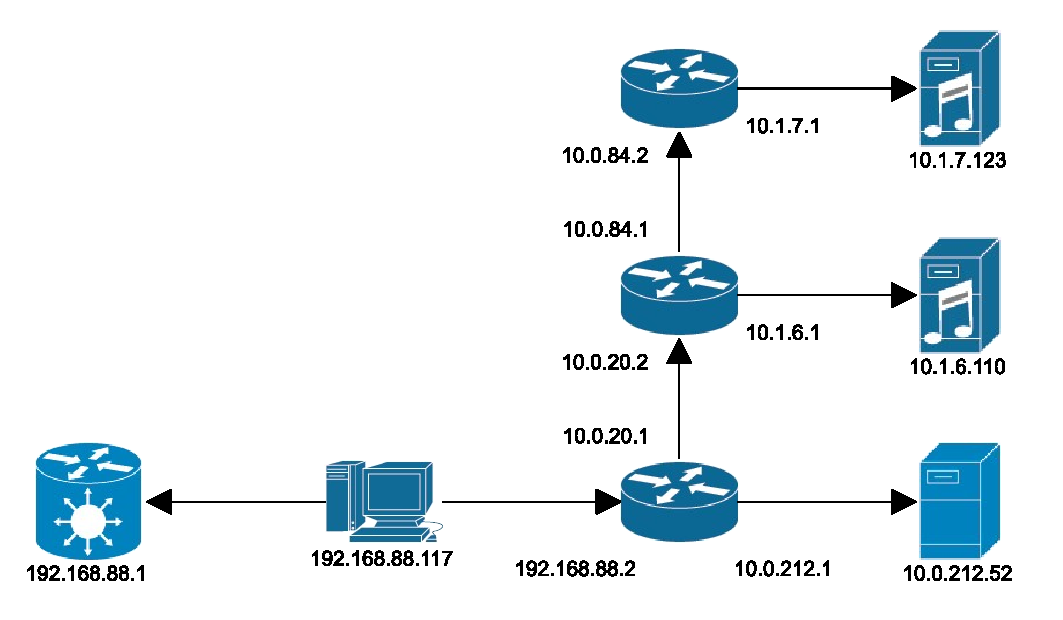
\includegraphics[width=\textwidth]{network_layout.pdf} 
    \caption{Diagram of the network and its different sub-networks}
    \label{fig:networkLayout}
\end{figure}
\subsection{Routing tables of the routers}

\begin{table}[hb]
    \centering
    \caption{Routing table for our network \#TODO Other directions}
    \label{tab:routing}
    \begin{tabular}{lll}
        \toprule
        \textbf{router} & \textbf{destination} & \textbf{via}  \\ \midrule
        r1 & 10.0.212.0/24 &  10.0.212.1 \\
        r1 & 10.1.6.0/24   &  10.0.20.2 \\
        r1 & 10.1.7.0/24   &  10.0.20.2 \\
        \midrule
        r2 & 10.1.6.0/24 & 10.1.6.1 \\
        r2 & 10.1.7.0/24 & 10.0.84.2 \\
        \midrule
        r3 & 10.1.7.0/24 & 10.1.7.1\\
        \bottomrule
    \end{tabular}
\end{table}

\subsection{Measured network parameters}

The \texttt{ping} and \texttt{mtrace} tools are used to obtain information on the network, especially for the Landline and Satellite hosts.
With \texttt{mtrace}, routers on the way of a packet are discovered by limiting the hop limit of the packet and listening for their expiration message.
Figures \ref{fig:mtraceLandline}, \ref{fig:mtraceSatellite} and Table \ref{tbl:mtraceResults} show the generated results.
We can observe a more severe packet loss on the routers that are between our host and our remote. 
As the packet loss is way lower for packets that shall reach the remote host, we assume that some kind of rate limiting process is taking place in the routers (i.e. router is dropping ICMP packets to save resources).
We observe that Landline experiences no packet loss while Satellite losses 4.2\% of its packets. 
This is the main reason for the degraded quality.

\begin{table}[hb]
    \centering
    \caption{Results from mtrace}
    \label{tbl:mtraceResults}
    \begin{tabular}{cccccc}
        \toprule
        Destination & Packet Loss [\%] & Avg [ms] & Best [ms] & Worst [ms] & Standard Deviation  \\ \midrule
        Satellite & 4.2 & 961.5 & 939.8 & 2694 & 58.9 \\
        Landline & 0 & 159.1 & 151.6 & 167.1 & 3.2\\
        \bottomrule
    \end{tabular}
\end{table}

\begin{figure}[ht]
    \centering
   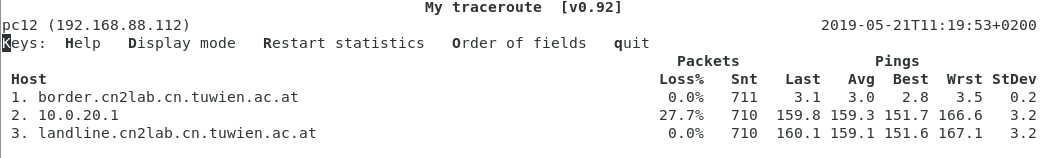
\includegraphics[width=\textwidth]{images/mytraceroute1.png} 
    \caption{mtrace to Satellite}
    \label{fig:mtraceSatellite}
\end{figure}

\begin{figure}[ht]
    \centering
   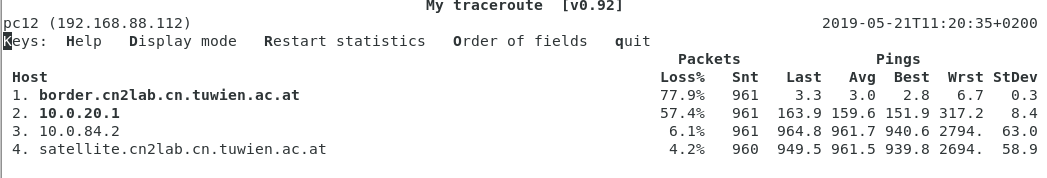
\includegraphics[width=\textwidth]{images/mytraceroute2.png} 
    \caption{mtrace to Landline}
    \label{fig:mtraceLandline}
\end{figure}


\begin{lstlisting}[language=tex, breaklines, frame=single, caption={Landline Network Parameters}, label=lst:landlineNetwork, float, floatplacement=h]
--- 10.1.7.123 ping statistics ---
2023 packets transmitted, 1902 received, 5.98122% packet loss, time 1004ms
rtt min/avg/max/mdev = 939.878/959.329/982.266/11.445 ms, pipe 5
\end{lstlisting}

\begin{lstlisting}[language=tex, breaklines, frame=single, caption={Landline Network Parameters}, label=lst:landlineNetwork, float, floatplacement=h]
--- 10.1.6.110 ping statistics ---
2364 packets transmitted, 2363 received, 0.0423012% packet loss, time 1105ms
rtt min/avg/max/mdev = 151.477/159.317/166.917/3.244 ms
\end{lstlisting}


\subsection{Graphical representation of the measured data (e.g. Histogram, CDF, ...)}
\subsection{Discussion of the results, comparing with the results from assignment 2}


%----------------------------------------------------------------------------------------
%	SECTION X
%---------------------------------------------------------------------------------------


%%%%%%%%%%%%%%%%%%%%%%%%%%%%%%%%%%%%%%%%%%%%%%%
\end{document}
